\documentclass[12pt,aspectratio=169]{beamer}

\mode<presentation>
{
  \usetheme{Singapore}
 %\setbeamersize{text margin left=.6cm,text margin right=.6cm}
%  \setbeamertemplate{navigation symbols}{} % suppress nav bar
%  \setbeamercovered{transparent}
}
\usefonttheme{professionalfonts}
%\usepackage{graphicx}
\usepackage{tikz}
\usepackage{amsmath,bm}
\usepackage{mathpazo}
\usepackage[scaled]{helvet}
\usepackage{xcolor,colortbl}
\usepackage{siunitx}
%\usepackage{hyperref}

\sisetup{detect-all}

\title{Class 20: Thermodynamics}
\subtitle{AP Physics}
\author[TML]{Dr.\ Timothy Leung}
\institute{Olympiads School}
\date{April 2018}

\newcommand{\pic}[2]{\includegraphics[width=#1\textwidth]{#2}}
\newcommand{\mb}[1]{\mathbf{#1}}
\newcommand{\eq}[2]{\vspace{#1}{\Large\begin{displaymath}#2\end{displaymath}}}

\begin{document}

\begin{frame}
  \maketitle
\end{frame}



\begin{frame}
  \frametitle{Files for You to Download}
  Download from the school website:
  \begin{enumerate}
  \item\texttt{20-thermodynamics.pdf}---This presentation. If you want to print
    the slides on paper, I recommend printing 4 slides per page.
  \item\texttt{20-Homework.pdf}---Homework assignment for Classes 19 and 20,
    which cover Fluid Mechanics and Thermodynamics
  \end{enumerate}

  \vspace{.2in}There are also three PDF files with supplemental information.
  Some of the information on those files are duplicates. Please download/print
  and read them.
\end{frame}



\begin{frame}
  \frametitle{Review: Absolute Temperature Scale}
  \framesubtitle{aka the Kelvin Scale}
  Relationship between the absolute temperature scale and the Celsius scale is
  a constant:
  
  \eq{-.4in}{
    \boxed{T = T_C + 273.15}
  }
  
  \vspace{-.1in}Plotting pressure vs.\ temperature at \emph{constant volume}
  for gases gives a straight line that appear to intersect the $x$-axis at
  \SI{-273.15}{\celsius}:
  \begin{center}
    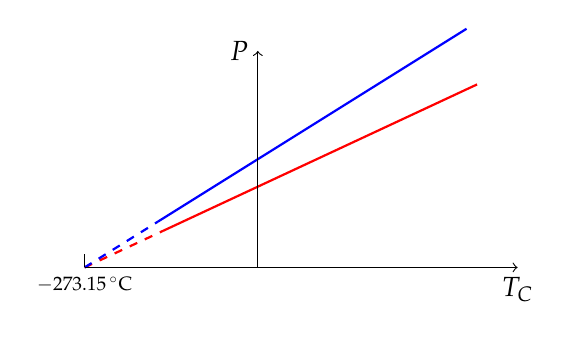
\begin{tikzpicture}[scale=1.1]
      \begin{scope}[rotate=25]
        \draw[thick,red,dashed](0,0)--(1,0);
        \draw[thick,red](1,0)--(5,0);
      \end{scope}
      \begin{scope}[rotate=32]
        \draw[thick,blue,dashed](0,0)--(1,0);
        \draw[thick,blue](1,0)--(5.2,0);
      \end{scope}
      \draw[->](0,0)--(5,0) node[pos=1,below]{$T_C$};
      \draw(0,0)--(0,.15) node[pos=0,below]{\scriptsize\SI{-273.15}{\celsius}};
      \draw[->](2,0)--(2,2.5) node[pos=1,left]{$P$};
    \end{tikzpicture}
  \end{center}
\end{frame}



\begin{frame}
  \frametitle{Review: Absolute Temperature Scale}
  \eq{.01in}{
    \boxed{T = T_C + 273.15}
  }
  \begin{center}
    \begin{tabular}{l|c|l}
      \rowcolor{pink}
      \textbf{Quantity}     & \textbf{Symbol} & \textbf{SI Unit} \\ \hline
      Absolute temperature  & $T$            & \si{\kelvin} (Kelvin) \\
      Temperature in degree Celsius & $T_C$  & \si{\celsius} is not an SI unit
    \end{tabular}
  \end{center}
  \begin{itemize}
  \item Developed by William Thomson (Lord Kelvin) and James Joule
  \item Until the 1960's, absolutely temperature used the unit ``degree kelvin''
  \item The temperature \emph{change} of \SI{1}{\kelvin} is the same as
    \SI{1}{\celsius}
  \item The two scales differ in where \emph{zero} is (called the
    ``null point'')
  \end{itemize}
\end{frame}
  

\begin{frame}
  \frametitle{Relationship Between Temperature and Pressure}
  The relationship between absolute temperature $T$ and pressure $P$
  of a gas at constant volume is defined using its triple point:

  \eq{-.1in}{
    T=\frac{T_\mathrm{tp}}{P_\mathrm{tp}}P
  }

  \textbf{Triple point} is a combination of pressure and temperature where all
  phases of a substance (solid, liquid and vapour) may coexist in thermal
  equilibrium.
  \begin{itemize}
  \item The triple point temperature for water is at
    $T_\mathrm{tp}=\SI{273.16}{\kelvin}$, or $\SI{0.01}{\celsius}$
  \item Triple point pressure for water is $P_\mathrm{tp}=\SI{611.2}{\pascal}$
  \end{itemize}
\end{frame}



\begin{frame}
  \frametitle{Thermal Expansion}
  When temperature $T$ of an object with length $L$ increases, the object
  \emph{usually} expands. The \emph{thermal strain} ($\Delta L/L$) is
  proportional the change in temperature:
  
  \eq{-.2in}{
    \boxed{\frac{\Delta L}{L} =\alpha\Delta T}\quad\text{\normalsize where}\quad
    \boxed{\alpha=\frac{1}{L}\frac{dL}{dT}}
  }
  \begin{center}
    \begin{tabular}{l|c|l}
      \rowcolor{pink}
      \textbf{Quantity} & \textbf{Symbol} & \textbf{SI Unit} \\ \hline
      Length      & $L$  & \si{\metre} (meter) \\
      Temperature & $T$  & \si{\kelvin} (kelvin)\\
      \textbf{Coefficient of linear expansion} & $\alpha$ &
      \si{\per\kelvin} (per kelvin)
    \end{tabular}
  \end{center}

  $\alpha$ is independent of pressure for solids and liquids, but may vary
  with $T$.
\end{frame}


\begin{frame}
  \frametitle{Thermal Expansion}
  There is also a similar expression for
  \textbf{coefficient of volume expansion}:
  
  \eq{-.2in}{
    \boxed{\frac{\Delta V}{V}=\beta\Delta T}
    \quad\text{\normalsize where}\quad
    \boxed{\beta=\frac{1}{V}\frac{dV}{dT}}
  }

  \vspace{-.05in}$\beta$ is also independent of pressure for solids and liquids,
  but may vary with $T$.
  \begin{center}
    \begin{tabular}{l|c|l}
      \rowcolor{pink}
      \textbf{Quantity} & \textbf{Symbol} & \textbf{SI Unit} \\ \hline
      Volume      & $V$  & \si{\m^3} (cube meter) \\
      Temperature & $T$  & \si{\kelvin} (kelvin)\\
      Coefficient of volume expansion & $\beta$ & \si{\per\kelvin} (per kelvin)
    \end{tabular}
  \end{center}

  Careful application of calculus will show that for isotropic material (where
  $\alpha$ is the same in all direction)

  \eq{-.45in}{
    \beta = 3\alpha
  }
\end{frame}



\begin{frame}
  \frametitle{Ideal Gas Law for Low-Density Gases}

  \textbf{Boyle's Law}: Physicist Robert Boyle (1627-1691) discovered that,
  when a gas is allowed to expand or compress at \emph{constant temperature},
  the product of pressure $P$ and $V$ remain constant, i.e.:

  \eq{-.2in}{
    PV=\textrm{constant} %\quad\quad\text{\normalsize constant temperature}
  }

  \vspace{-.1in}We also know that at \emph{constant volume}, temperature is
  proportional to pressure. This is how we got the absolute temperature scale
  discussed earlier, i.e.:

  \eq{-.3in}{
    PV=CT
  }

  \vspace{-.2in}where ``C'' is some constant to be determined.
\end{frame}


\begin{frame}
  \frametitle{Ideal Gas Law}
  Thought experiment:
  \begin{itemize}
  \item Two identical containers with volume $V$ with same amount of same kind
    of gas at same pressure $P$ and temperature $T$.
  \item When the containers are combined and the molecules are free to
    move, $P$ and $T$ remain the same, but volume is increased by factor of 2.
  \end{itemize}

  $C$ must scale with the number of molecules of gas $N$, which modifies the
  equation to this, the \textbf{ideal gas law}:

  \eq{-.25in}{
    \boxed{PV=NkT}
  }

  \vspace{-.15in}The constant $k=\SI{1.381e-23}{\joule/\kelvin}$ is called
  \textbf{Boltzmann's constant}. It is found experimentally to have the same
  value for any kind or amount of gas.
\end{frame}



\begin{frame}
  \frametitle{Ideal Gas Law}
  The ideal gas law can also be written a more familiar way:
  %The ideal gas law is more often written in terms of the number of
  %\emph{moles} of gas $n$ and the \textbf{universal gas constant} $R$:
  
  \eq{-.2in}{
    \boxed{PV=nRT}
  }

  \vspace{-.25in}where
  \begin{itemize}
  \item $n=N/N_A$ is the number of moles of the gas
  \item $R=kN_A=\SI{8.314}{\kilo\gram/\mol.\kelvin}$ is the universal gas
    constant, and
  \item $N_A=\num{6.022e23}$ is Avagadro's number
  \end{itemize}

  \vspace{.1in}The ideal gas law is an \emph{equation of state}, because it
  relates all the quantities that define the \emph{state} of a gas: pressure
  $P$, volume $V$ and temperature $T$.
\end{frame}


\begin{frame}
  \frametitle{Kinetic Theory of Gases}
  Assumptions for the kinetic theory of gases:
  \begin{enumerate}
  \item The gas consists of a large number of molecules that make
    \emph{elastic} collisions with each other and with the walls of the
    container.
  \item The molecules are separated, on average, by distances that are large
    compared to their diameters, and they exert no force (gravitational,
    electrostatic etc) on each other except when they collide.\footnotemark
  \item In the absence of external forces, there is no preferred position for a
    molecules in the container, and there is no preferred velocity vector.
  \end{enumerate}

  \footnotetext[1]{This means that the density of the gas is low, i.e. assume
    ideal gas behaviour.}
\end{frame}


\begin{frame}
  \frametitle{Average Kinetic Energy of a Gas}
  We note that pressure is force of the gas molecules exerts when colliding
  with the container, given by

  \eq{-.3in}{ P=\frac{F}{A} }

  By Newton's second law of motion: the collision changes the momentum of the
  gases

  \eq{-.3in}{ \mb{F}=\frac{d\mb{p}}{dt} }

  We can then relate the change momentum, to force to pressure and to the ideal
  gas law. After some calculus\ldots
\end{frame}

\begin{frame}
  \frametitle{Average Kinetic Energy of a Gas}
  We find the average kinetic energy $\langle K \rangle$ of a molecule of gas
  in a container, given by:
  
  \eq{-.2in}{
    \boxed{\big\langle K\big\rangle=\frac{3}{2}kT}
  }

  \vspace{-.1in}i.e.\ temperature is a measurement of the average kinetic
  energy.

  \vspace{.15in}Often it is advantageous to calculate the root mean square
  (``rms'') velocity of the molecules, which measures the speeds that the
  majority of the particles are below:

  \eq{-.2in}{
    v_\mathrm{rms}=\sqrt{\frac{3kT}{m}}
  }
\end{frame}


\begin{frame}
  \frametitle{$P$-$V$ Diagram}
  Thermodynamic processes is usually plotted on a ``$P$-$V$ diagram''.
  \begin{columns}

    \column{.35\textwidth}
    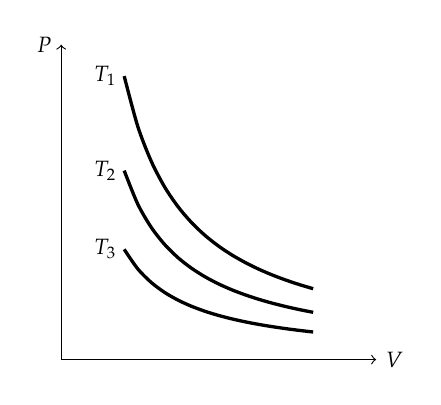
\begin{tikzpicture}[scale=.8]
      \draw[->](0,0)--(5,0) node[pos=1,right]{\footnotesize $V$};
      \draw[->](0,0)--(0,5) node[pos=1,left]{\footnotesize $P$};
      \draw[smooth,samples=15,domain=1:4,very thick] plot({\x},{1.75/\x});
      \draw[smooth,samples=15,domain=1:4,very thick] plot({\x},{3/\x});
      \draw[smooth,samples=15,domain=1:4,very thick] plot({\x},{4.5/\x});
      \node (t1) at (.7,1.75){\footnotesize $T_3$};
      \node (t1) at (.7,3)   {\footnotesize $T_2$};
      \node (t1) at (.7,4.5) {\footnotesize $T_1$};
    \end{tikzpicture}

    \column{.65\textwidth}
    \begin{itemize}
    \item Under constant temperature, the relationship between pressure and
      volume is a hyperbolic curve.
    \item Each line is called an \textbf{isotherm}; it represents a different
      constant temperature
    \item $T_3>T_2>T_1$
    \end{itemize}
  \end{columns}
  
  \vspace{.2in}{\footnotesize\textbf{Note:} Aside from $P$-$V$ diagrams, there
    are many similar diagrams in thermodynamics. \par}
\end{frame}


\begin{frame}
  \frametitle{Real Gases}
  Most gases behave like ideal gas at most ordinary pressures, but the
  equation breaks down when the density of gas is high and molecules are not
  far apart:
  \begin{itemize}
  \item pressure is sufficiently high
  \item temperature is low
  \end{itemize}
  In this situation the \textbf{van der Waal equation} provides a more accurate
  description of the behaviour of real gases:

  \eq{-.2in}{
    \boxed{\left(P+\frac{an^2}{V^2}\right)(V-bn)=nRT}
  }

  \begin{itemize}
  \item The term $an^2/V^2$ is from the attraction of the gas molecules to each
    other
  \item The term $b$ is approximately the volume occupied by one mole of the gas
  \end{itemize}
\end{frame}




\begin{frame}
  \frametitle{Real Substances}
  Neither the \textbf{ideal gas law} nor the \textbf{van der Waal equation}
  can capture the exact relationship between pressure and volume, because
  neither can account for phase changes. The $P$-$V$ diagram of a real substance
  is like this:
  \begin{center}
    \pic{.35}{realsubstance.jpg}
  \end{center}
\end{frame}


\begin{frame}
  \frametitle{Phase Diagrams}
  The phase diagram plots pressure against temperature to show when the
  different phases of matter exist. For water:
  \begin{center}
    \vspace{-.1in}
    \pic{.4}{10-figure-31.png}
  \end{center}
  \begin{itemize}
  \item\vspace{-.15in} At \textbf{triple point} $B$, all three phases of matter
    can exist in equilibrium
  \item At \textbf{critical point} $C$, liquid and vapour (gas) are
    indistinguishable, and the gas laws can model their behaviour
  \end{itemize}
\end{frame}


\begin{frame}
  \frametitle{First Law of Thermodynamics}
  \begin{block}{First Law of Thermodynamics}
    The change in the internal energy of a system is the sum of the work and
    heat exchanged between a system and its surroundings. 
  \end{block}
  
  \eq{-.2in}{
    \boxed{\Delta U=Q-W}
  }
  %\vspace{.1in}
  \begin{center}
    \begin{tabular}{l|c|l}
      \rowcolor{pink}
      \textbf{Quantity} & \textbf{Symbol} & \textbf{SI Unit} \\ \hline
      Change in internal energy of a system & $\Delta U$ & \si{J} (joules) \\
      Work done by the system      & $W$                 & \si{J} (joules) \\
      Heat into the system         & $Q$                 & \si{J} (joules)
    \end{tabular}
  \end{center}

  \textbf{IMPORTANT NOTE:} Sometimes the equation is written as
  $\Delta U=Q+W$, where $W$ is the work done \emph{to} the system, rather
  than \emph{by} the system. Both conventions are commonly use. You have to
  be very careful.
\end{frame}


\begin{frame}
  \frametitle{First Law of Thermodynamics}
  \vspace{-.2in}{\LARGE
    \begin{displaymath}
      \boxed{\Delta U=Q-W}
    \end{displaymath}
  }
  
  Internal energy $U$ is the sum of kinetic and potential energies, but does
  \emph{not} include
  \begin{itemize}
  \item The bulk kinetic energy of the system, i.e.\ if the entire container
    of gas moves at speed $v$
  \item The potential energy inside a force field, e.g.\ gravitational,
    electrostatic, magnetic
  \end{itemize}
  For an ideal gas, the internal energy is just the total kinetic energy of the
  gas:

  \eq{-.2in}{
    U=K=\frac{1}{2}NkT=\frac{1}{2}nRT
  }
\end{frame}



\begin{frame}
  \frametitle{First Law of Thermodynamics}
  \vspace{-.2in}{\LARGE
    \begin{displaymath}
      \boxed{\Delta U=Q-W}
    \end{displaymath}
  }

  \begin{columns}
    \column{.7\textwidth}
    $Q$ is the \emph{thermal energy} (heat) \emph{into} the system, through
    conduction, convection and radiation.
    \begin{itemize}
    \item $+$ if heat is added to the system
    \item $-$ if heat leaves the system
    \end{itemize}

    For conduction, the rate of heat transfer $\Delta Q/\Delta t$ (aka ``thermal
    current'') is given by:

    \eq{-.2in}{
      \boxed{H=\frac{\Delta Q}{\Delta t}=kA\frac{\Delta T}{\Delta x}}
    }

    \vspace{-.15in}where $k$ is the thermal conductivity of the material

    \column{.3\textwidth}
    \pic{1}{conduct.png}
    \end{columns}
\end{frame}



\begin{frame}
  \frametitle{First Law of Thermodynamics}
  \vspace{-.2in}{\LARGE
    \begin{displaymath}
      \boxed{\Delta U=Q-W}
    \end{displaymath}
  }

  \vspace{-.1in}$W$ is the mechanical work done by the system to the surrounding
  \begin{itemize}
  \item $+$ done by the system, e.g.
    %\begin{itemize}
    %\item
    Using steam pressure to push a piston or shaft
    %\end{itemize}
  \item $-$ done \emph{to} the system, e.g.
    %\begin{itemize}
    %\item
    pushing a piston to compress gas in an engine
    %\item Joule's experiment: stirring water to raise its temperature
    %\end{itemize}
  \end{itemize}
%\end{frame}
%
%
%
%\begin{frame}
%  \frametitle{Work Done To a Gas}
%  The work done \emph{on} an ideal gas is:

  \eq{-.2in}{
    \boxed{ W=\int_{P_1}^{P_2} PdV}
  }
  
  \vspace{-.1in}It's up to you to show that this equation is derived from the
  definition of work, $W=\int\mb{F}\cdot d\mb{s}$.
\end{frame}

\begin{frame}
  \frametitle{Work Done To a Gas}
  On the $P$-$V$ diagram, $W$ is the area under the curve.
  \begin{itemize}
  \item $W$ is done \emph{by} the system (positive) if the path moves right, and
  \item done \emph{to} the system (negative) if it moves left
  \end{itemize}

  In the example below, the gas is changed from point 1 to 2, but the work done
  is different.
  \begin{center}
    \vspace{-.1in}
    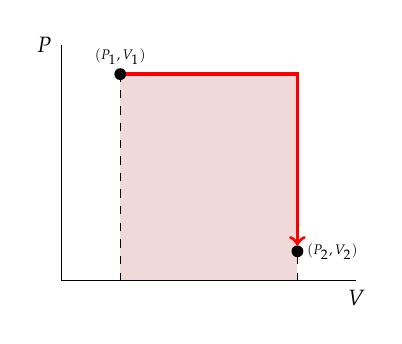
\begin{tikzpicture}[scale=.75]
      \fill[pink!80!gray!50](1,0) rectangle(4,3.5);
      \draw[dashed](1,0)--(1,3.5);
      \draw[dashed](4,0)--(4,.5);
      \draw(0,0)--(5,0) node[pos=1,below]{\footnotesize $V$};
      \draw(0,0)--(0,4) node[pos=1,left]{\footnotesize $P$};
      \draw[very thick,->,red](1,3.5)--(4,3.5)--(4,.6);
      \fill[black](1,3.5) circle(.1) node[above]{\tiny $(P_1,V_1)$};
      \fill[black](4,.5) circle(.1)  node[right]{\tiny $(P_2,V_2)$};
    \end{tikzpicture}
    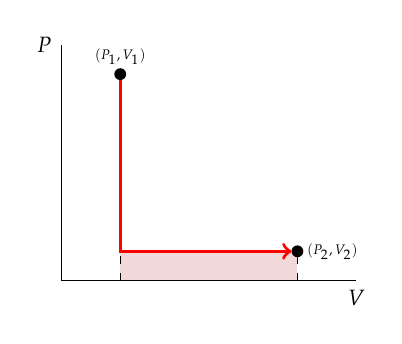
\begin{tikzpicture}[scale=.75]
      \fill[pink!80!gray!50](1,0) rectangle(4,.5);
      \draw[dashed](1,0)--(1,3.5);
      \draw[dashed](4,0)--(4,.5);
      \draw(0,0)--(5,0) node[pos=1,below]{\footnotesize $V$};
      \draw(0,0)--(0,4) node[pos=1,left]{\footnotesize $P$};
      \draw[very thick,->,red](1,3.5)--(1,.5)--(3.9,.5);
      \fill[black](1,3.5) circle(.1) node[above]{\tiny $(P_1,V_1)$};
      \fill[black](4,.5) circle(.1)  node[right]{\tiny $(P_2,V_2)$};
    \end{tikzpicture}
    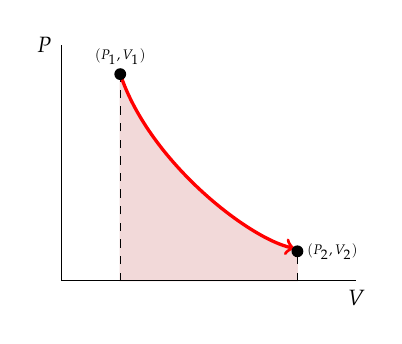
\begin{tikzpicture}[scale=.75]
      \draw[fill=pink!80!gray!50,draw=pink!80!gray!50]
      (1,0)--(1,3.5)..controls(1.5,2) and (3.2,.7)..(4,.5)--(4,0)--cycle;
      \draw[dashed](1,0)--(1,3.5);
      \draw[dashed](4,0)--(4,.5);
      \draw(0,0)--(5,0) node[pos=1,below]{\footnotesize $V$};
      \draw(0,0)--(0,4) node[pos=1,left]{\footnotesize $P$};
      \draw[very thick,->,red](1,3.5)..controls(1.5,2) and (3.2,.7)..(3.95,.55);
      \fill[black](1,3.5) circle(.1) node[above]{\tiny $(P_1,V_1)$};
      \fill[black](4,.5) circle(.1)  node[right]{\tiny $(P_2,V_2)$};
    \end{tikzpicture}
  \end{center}
\end{frame}



\begin{frame}
  \frametitle{Quasi-Static Processes}

  
  In thermodynamics, a \textbf{quasi-static process} is a thermodynamic process
  that happens slowly enough for the system to remain in internal equilibrium.
  We are concerned with 4 of these process:
  \begin{itemize}
  \item Isobaric process - constant pressure
  \item Isochoric process - constant volume
  \item Isothermal process - constant temperature
  \item Adiabatic process - ``isolated'', no heat exchanged with surrounding
  \end{itemize}
\end{frame}

\begin{frame}
  \frametitle{Quasi-Static Processes}
  \begin{center}
    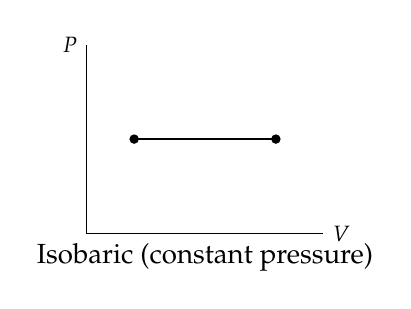
\begin{tikzpicture}[scale=.6]
      \draw(0,0)--(5,0) node[pos=1,right]{\footnotesize $V$}
      node[midway,below]{Isobaric (constant pressure)};
      \draw(0,0)--(0,4) node[pos=1,left]{\footnotesize $P$};
      \draw[thick](1,2)--(3.95,2);
      \fill[black](1,2) circle(.1);
      \fill[black](4,2) circle(.1);
    \end{tikzpicture}
    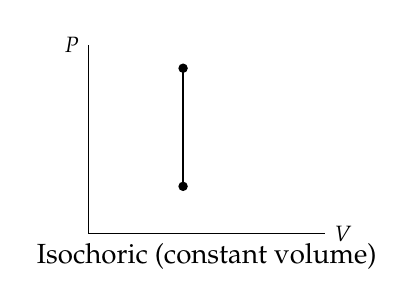
\begin{tikzpicture}[scale=.6]
      \draw(0,0)--(5,0) node[pos=1,right]{\footnotesize $V$}
      node[midway,below]{Isochoric (constant volume)};
      \draw(0,0)--(0,4) node[pos=1,left]{\footnotesize $P$};
      \draw[thick](2,1)--(2,3.5);
      \fill[black](2,1)   circle(.1);
      \fill[black](2,3.5) circle(.1);
    \end{tikzpicture}
    
    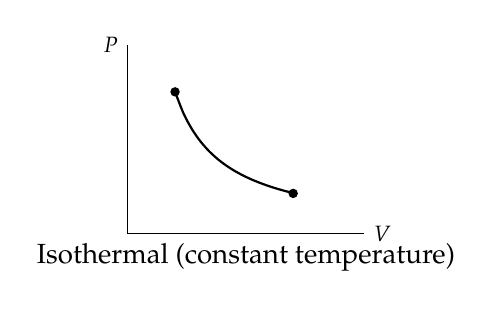
\begin{tikzpicture}[scale=.6]
      \draw(0,0)--(5,0) node[pos=1,right]{\footnotesize $V$}
      node[midway,below]{Isothermal (constant temperature)};
      \draw(0,0)--(0,4) node[pos=1,left]{\footnotesize $P$};
      \draw[smooth,samples=15,domain=1:3.5,thick] plot({\x},{3/\x});
      \fill[black](1,3)   circle(.1);
      \fill[black](3.5,.85) circle(.1);
    \end{tikzpicture}
    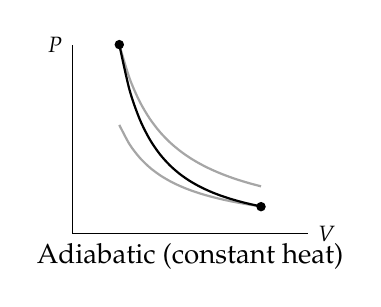
\begin{tikzpicture}[scale=.6]
      \draw(0,0)--(5,0) node[pos=1,right]{\footnotesize $V$}
      node[midway,below]{Adiabatic (constant heat)};
      \draw(0,0)--(0,4) node[pos=1,left]{\footnotesize $P$};
      \draw[smooth,samples=15,domain=1:4,thick,gray!70] plot({\x},{4/\x});
      \draw[smooth,samples=15,domain=1:4,thick,gray!70] plot({\x},{2.3/\x});
      \draw[smooth,samples=15,domain=1:4,thick] plot({\x},{4*((\x)^(-1.4))});
      \fill[black](1,4) circle(.1);
      \fill[black](4,.57) circle(.1);
    \end{tikzpicture}
  \end{center}
\end{frame}



\begin{frame}
  \frametitle{A Simple Heat Engine Cycle}
  \begin{columns}
    \column{.8\textwidth}
    \begin{center}
      \pic{.5}{heat-engine.jpg}
    \end{center}
    \begin{enumerate}
    \item\vspace{-.15in} Heat is added at constant volume; no work done.
    \item Heat is added as gas expands at constant pressure; work is done by
      the gas to lift the weight.
    \item Heat is extracted at constant volume; no work done.
    \item Heat is extracted at constant pressure; work is done on the gas to
      compress it.
    \end{enumerate}
    \column{.2\textwidth}
    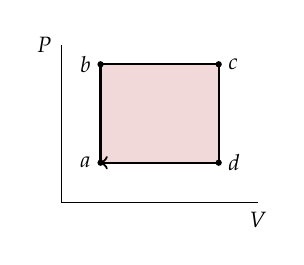
\begin{tikzpicture}[scale=.5]
      \fill[pink!80!gray!50](1,1) rectangle(4,3.5);
      \draw(0,0)--(5,0) node[pos=1,below]{\footnotesize $V$};
      \draw(0,0)--(0,4) node[pos=1,left]{\footnotesize $P$};
      \draw[thick,->](1,1)--(1,3.5)--(4,3.5)--(4,1)--(1,1);
      \fill[black](1,1) circle(.08) node[left]{\footnotesize$a$};
      \fill[black](1,3.5) circle(.08) node[left]{\footnotesize$b$};
      \fill[black](4,3.5) circle(.08) node[right]{\footnotesize$c$};
      \fill[black](4,1) circle(.08) node[right]{\footnotesize$d$};
    \end{tikzpicture}

    {\footnotesize $P$-$V$ diagram of the simple heat engine shown on the left.
      \par}
  \end{columns}
\end{frame}


\begin{frame}
  \frametitle{Efficiency of Heat Engine}
  In a heat engine, the internal energy at the beginning and end of the cycle
  are the same (same point on the $P$-$V$ diagram), so the work done is just
  the difference between heat added and taken out:
  
  \eq{-.25in}{
    W = Q_\mathrm{in}-Q_\mathrm{out}
  }
  
  \vspace{-.15in}Efficiency is defined as the ratio between work done and heat
  added:

  \eq{-.25in}{
    \boxed{\eta =\frac{W}{Q_\mathrm{in}}=1-\frac{Q_\mathrm{out}}{Q_\mathrm{in}}}
  }

  %So, you \emph{can} have a \SI{100}{\percent} efficient heat engine, but then
  %the engine will not do any work.
\end{frame}


\begin{frame}
  \frametitle{Second Law of Thermodynamics}


  \begin{block}{Kelvin-Planck Statement}
    It is impossible for heat engine working in a cycle to produce no other
    effect than that of extracting heat from a reservoir and performing an
    equivalent amount of work.
  \end{block}
\end{frame}

\begin{frame}
  \frametitle{Carnot Engine}
  The Carnot engine cycle is the most efficient.
  \begin{center}
    \pic{.4}{carnot.jpg}
  \end{center}
  The efficiency of a Carnot engine is:
  
  \eq{-.25in}{
    \boxed{\eta_C =1-\frac{Q_\mathrm{out}}{Q_\mathrm{in}}=1-\frac{T_h}{T_c}}
  }
\end{frame}

\end{document}
